\subsection{GeneNetWeaverPhos}
\begin{frame}{GeneNetWeaverPhos}
\label{sec:gnw_extension}
Java program GeneNetWeaver extended in Julia as GeneNetWeaverPhos. Added activated protein concentration, in some cases equal to phosphorylated concentration.
% GeneNetWeaver simulates gene expression levels for biological networks so network inference methods can systematically be benchmarked and compared.
% The software is not sufficient to benchmark a network inference method for indirect protein kinase interactions since the underlying simulation method is a gene regulation model only taking transcription factors into account.
% The program was extended to take indirect kinase effects into account in simulating the gene expression levels.
% The software is an open source Java program with a vast amount of features and built-in datasets. The core code was rewritten in Python to make the process of extending it as easy as possible.
% Code from \texttt{HillGene.java} was used for gene regulation, and initial conditions are described in \texttt{SteadyStateExperiment.java}. 
% The effects from kinases are added to the model with the differential equations in~\autoref{eq:gnw_kinase}, that based on the equations described in \autoref{sec:Heinrich}.
% The model described in \autoref{sec:dream} is extended by replacing the protein level terms $p_i$ with $y_i \cdot p_i$ describing the effective level of each protein instead of the total amount.
% The model of GeneNetWeaver is nondimensionalized, $p_i$ does not describe an absolute concentration but is relative to a maximum concentration. $y_i \cdot p_i$ is also nondimensionalized, since $y_i$ is unitless~(\autoref{eq:y_i}).
\begin{subequations}
\label{eq:gnw_kinase}
\begin{align}
\label{eq:dydt}
\dv{\boldsymbol{\psi}}{t} &= \left(W_{\text{KP}+} \boldsymbol{\psi}_\text{KP} + \boldsymbol{\lambda}_+\right) \left( \boldsymbol{p}_\text{TFKP} - \boldsymbol{\psi} \right) - \left(W_{\text{KP}-} \boldsymbol{\psi}_\text{KP} + \boldsymbol{\lambda}_- \right) \boldsymbol{\psi}
\end{align}
\end{subequations}
% Here, $\dv{\phi_i}{t}$ is found using \autoref{eq:kinase_general}.
% The values $y_i$ describe the phosphorylated fraction of protein $i$, so in this model it is assumed that the phosphorylated version of any protein is the active version. This is a simplification, but enough of an extension as a starting point to include effect of the kinases in the simulation.
% The differential equation \autoref{eq:dydt} is used as well as the already mentioned ones~(\autoref{eq:gnw_main}) for simulation of system until approximate convergence.
% The initial conditions is the same as for GeneNetWeaver with the addition of using $y_i = 0.5$ for all $i$. 
% RNA log fold-change measurements used as node values are simulated by solving the ODE at different times $t$ using the function \texttt{integrate.odeint} from the Python package \texttt{SciPy}. 
% Individual simulations are run using a wildtype network, as well as networks lacking nodes based on each of the experimental knockout conditions. For knockouts, a node $i$ is removed from the graph by setting the maximum transcription rate of gene $i$ to zero, which is $m_i^{(RNA)} = 0$~(\autoref{eq:gnw_main.a}).
% Log fold-change values are calculated for each of the modified networks relative to the wildtype measurements, after simulation completion. The last and second-to-last measurements are checked for approximate convergence with \autoref{eq:convergence} using threshold $\epsilon_{tol} = 0.005$. Warnings from the \texttt{odeint} call are also used in determination of successful convergence. The ODE is first solved for times $t \in \{0,1,...,9\}$, if this fails to converge it is solved for $t \in \{0,10,...,90\}$ and lastly for $t \in \{0,100,...,900\}$. If all fails the regulation modules are setup anew, as well as setting model parameters with new random values.
GeneNetWeaver $f$ changed from using $\boldsymbol{p}$ to $\boldsymbol{\psi}$.
\begin{subequations}
\begin{align}
\dv{r_i}{t} &=
m_i^{(\text{RNA})} f_i(\textcolor{red}{\boldsymbol{\psi}}) - \lambda_i^{(\text{RNA})} r_i
\end{align}
\end{subequations}
% $\odot$ = element-wise multiplication
\end{frame}


\begin{frame}{Small example network}
\begin{columns}
\begin{column}{0.4\linewidth}

(A) True network.\\
(B-F) Red = KO. Node value = Simulated mRNA logFC. Edge value = true weight.\\
(G) Total effects.\\
(H) Inferred edge weights.\\


\end{column}
\begin{column}{0.6\linewidth}
\begin{figure}[ht]
\centering
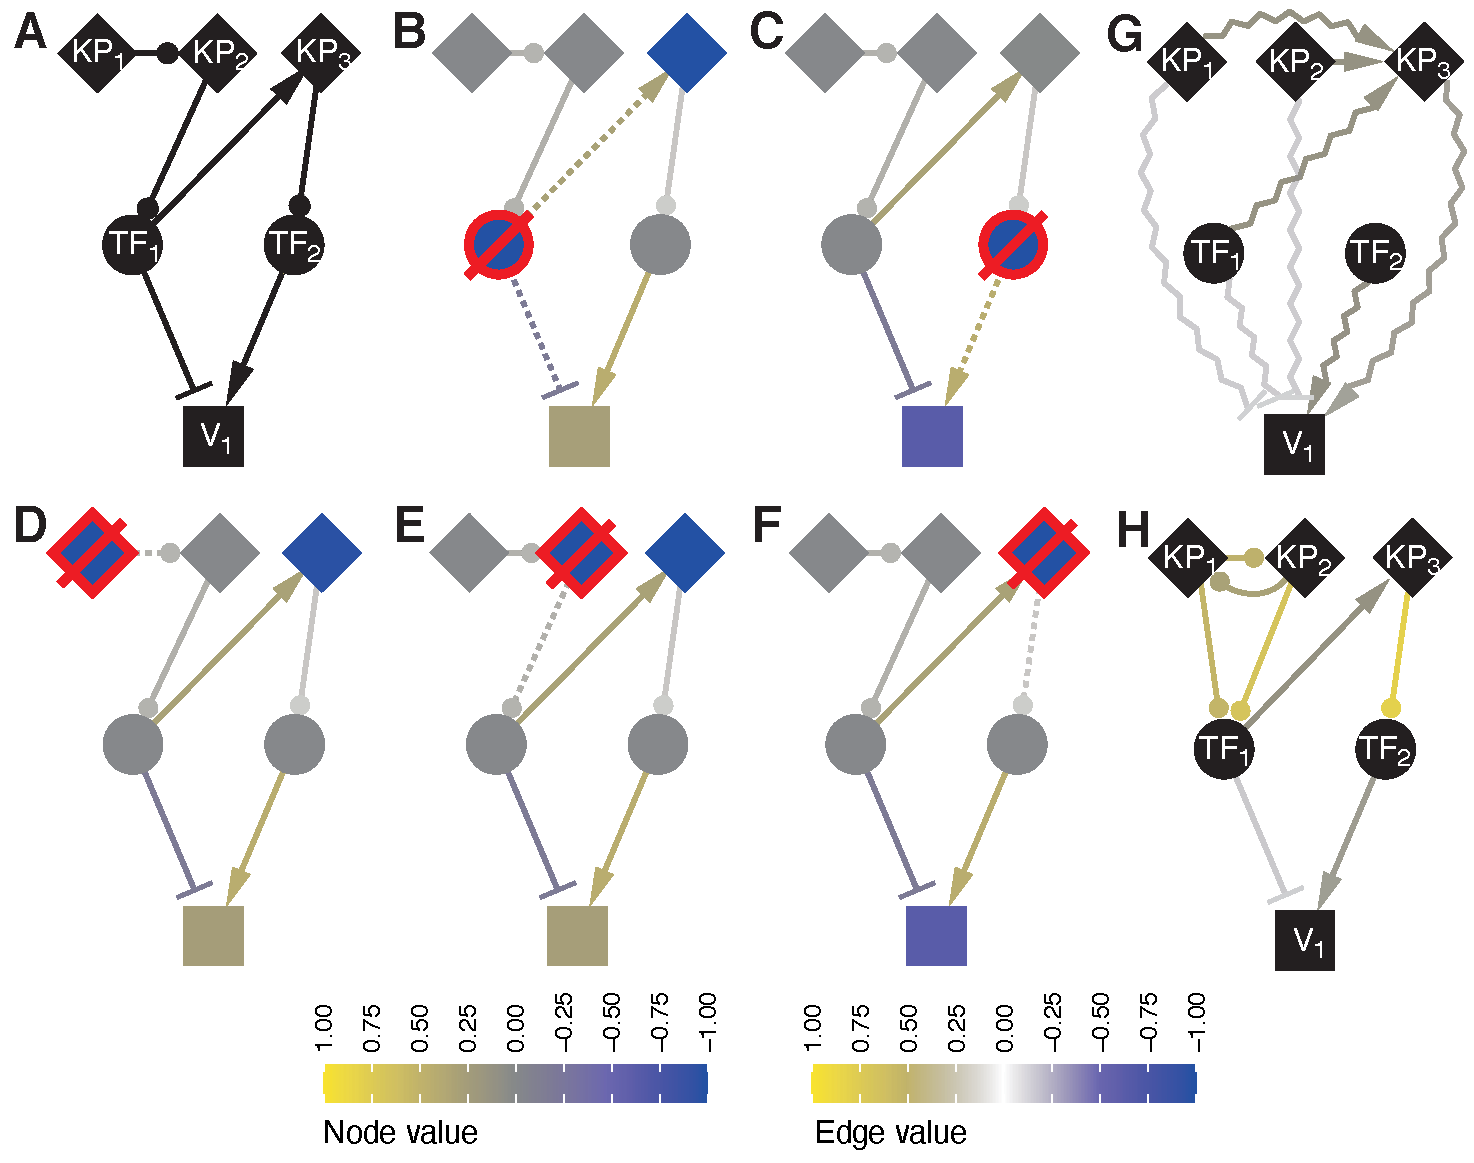
\includegraphics[width=\linewidth]{theory/fig/Fig2.pdf}
\caption{\textbf{Small example network with unresolvable ambiguity.}}
\label{fig:small}
\end{figure}
\end{column}
\end{columns}
\end{frame}


\begin{frame}{GeneNetWeaverPhos example}

\begin{columns}
\begin{column}{0.3\textwidth}
\end{column}
\begin{column}{0.7\textwidth}
\begin{figure}[ht]
    \centering
    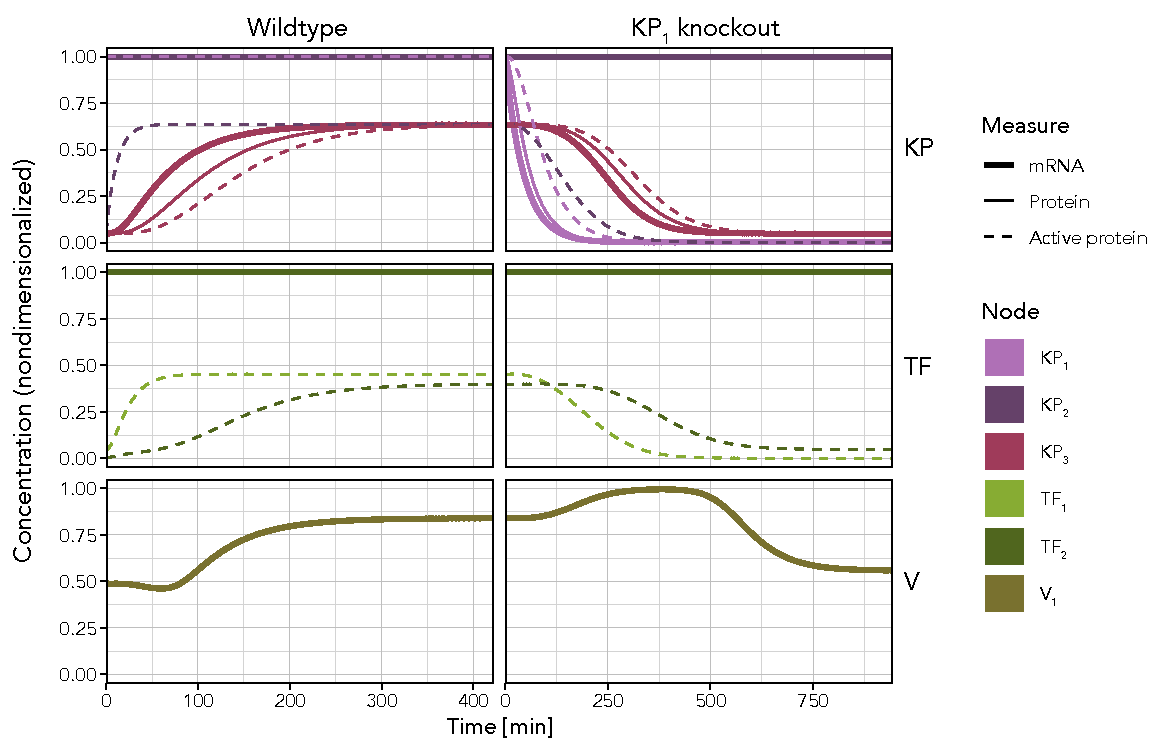
\includegraphics[width=\linewidth]{methods/fig/simulation_KP1_v4.pdf}
    \caption{{\bf Simulation until steady state.}
    Simulation of network in Fig~\ref{fig:small} in the main~text until convergence. 
    Comparing wildtype and a mutant where $\text{KP}_1$ has been knocked out. The values at convergence are seen in Fig~\ref{fig:small}D.
    }
     \label{fig:simulation}
\end{figure}
\end{column}
\end{columns}

\end{frame}

